\documentclass{article}
\usepackage{tikz}
\usetikzlibrary{arrows.meta}

\begin{document}

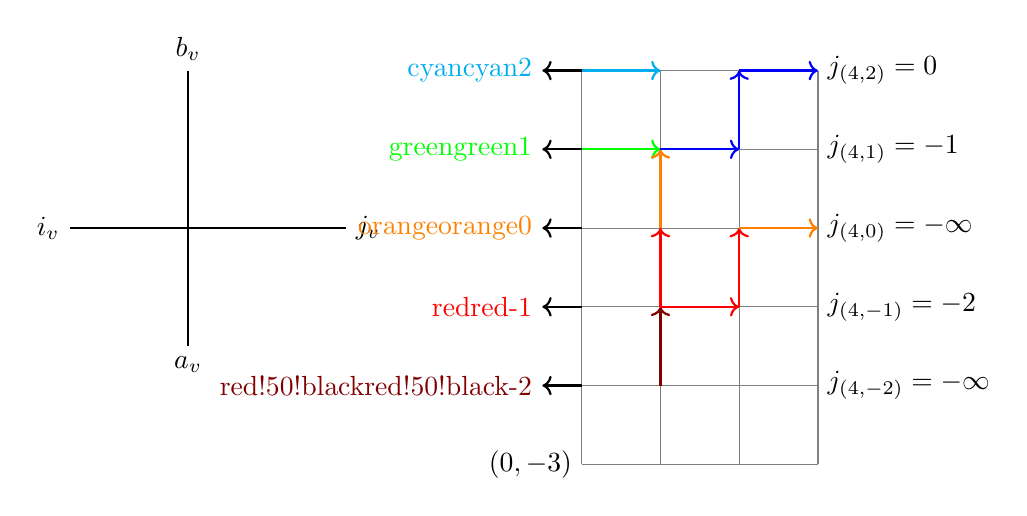
\begin{tikzpicture}
    % Left part: arrow configuration at a vertex v
    \draw[thick] (0, 0) -- (0, 2) node[above] {$b_v$};
    \draw[thick] (0, 0) -- (2, 0) node[right] {$j_v$};
    \draw[thick] (0, 0) -- (0, -1.5) node[below] {$a_v$};
    \draw[thick] (0, 0) -- (-1.5, 0) node[left] {$i_v$};
    
    % Right part: sample configuration of the colored stochastic six-vertex model
    \begin{scope}[xshift=5cm]
        % Grid lines
        \foreach \x in {0, 1, 2, 3} {
            \draw[gray] (\x, -3) -- (\x, 2);
        }
        \foreach \y in {-3, -2, -1, 0, 1, 2} {
            \draw[gray] (0, \y) -- (3, \y);
        }
        
        % Arrows and labels
        % Left boundary
        \foreach \y/\color in {2/cyan, 1/green, 0/orange, -1/red, -2/red!50!black} {
            \draw[->, \color, thick] (0, \y) -- (-0.5, \y) node[left] {\y};
        }
        \node[left] at (0, -3) {$(0, -3)$};
        
        % Colored arrows
        \draw[->, green, thick] (0,1) -- (1,1);
        \draw[->, cyan, thick] (0,2) -- (1,2);
        \draw[->, orange, thick] (1,0) -- (1,1);
        \draw[->, red, thick] (1,-1) -- (1,0);
        \draw[->, red!50!black, thick] (1,-2) -- (1,-1);
        \draw[->, red, thick] (1,-1) -- (2,-1);
        \draw[->, blue, thick] (1,1) -- (2,1);
        \draw[->, red, thick] (2,-1) -- (2,0);
        \draw[->, blue, thick] (2,1) -- (2,2);
        \draw[->, orange, thick] (2,0) -- (3,0);
        \draw[->, blue, thick] (2,2) -- (3,2);
        
        % Labels
        \node[right] at (3,2) {$j_{(4,2)} = 0$};
        \node[right] at (3,1) {$j_{(4,1)} = -1$};
        \node[right] at (3,0) {$j_{(4,0)} = -\infty$};
        \node[right] at (3,-1) {$j_{(4,-1)} = -2$};
        \node[right] at (3,-2) {$j_{(4,-2)} = -\infty$};
    \end{scope}
\end{tikzpicture}

\end{document}